\section{Testing eBPF programs}\label{sec:testing}
To verify the correctness of a P4-XDP program, the compiler integrates a full
end-to-end testing framework. The framework consists of an user space eBPF
runtime as well as a kernel testing pipeline, which verifies eBPF/XDP programs
in a virtual, isolated environment.

\subsection{Why Test in User-Space?}
Testing in user space isolates the specification of the eBPF program from the
implementation. It is primarily intended to test the correctness of the
compiler and the generated C code without interference of the kernel verifier
and tooling. The user space testing framework does not depend on the LLVM
compiler or specific kernel version. It also does not require usage of iproute2 
tools such as tc or ip. Our aim is to ensure that a P4 program is functionally
equivalent to its corresponding XDP C-code.
Testing in user space also guarantees debugging simplicity for the average
user. Debugging tools such as GDB, valgrind, wireshark, or simple statements
are readily available.

\subsection{The Simple Test Framework}
\begin{figure}
	\centering
	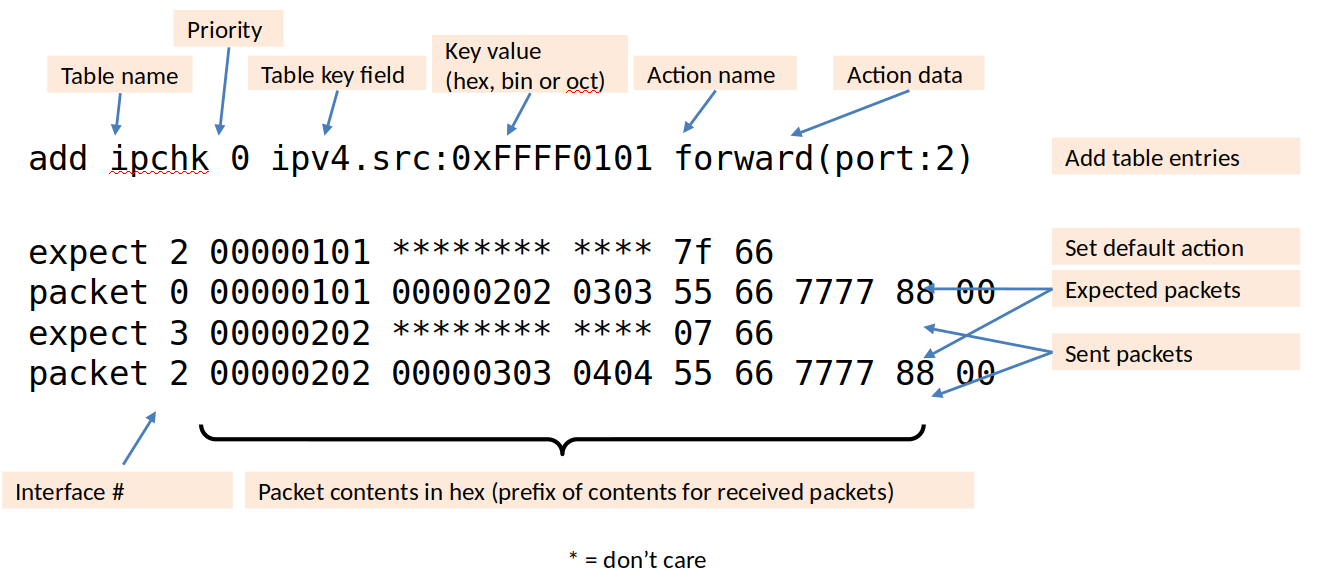
\includegraphics[width=\linewidth]{stf}
	\caption{Simple testing framework program fragment for exercising P4 programs.}
	\label{fig:stf}
\end{figure}
The simple test framework (STF) is a data plane verification language. 
An STF template defines a set of actions which are sequentially executed on the 
data plane.
The action \texttt{packet}, which describes an inbound Ethernet frame and the 
associated port number. The counterpart of \texttt{packet} is \texttt{expect}, 
which defines an outbound data frame. \texttt{add} emulates a data plane update 
by the control plane.

While its original purpose is to assess switching and forwarding behavior, it 
can also be used to test eBPF programs in isolation. The P4 compiler features a 
STF parser, which pre-processes the templates and provides an ordered command 
list. This command list is interpreted by the eBPF testing framework to run and 
execute end-to-end test.

\paragraph{Example}
An example can be seen in Figure \ref{fig:stf}. \texttt{add} defines that, if 
the IPv4 source address of a 
packet matches with the key in table \texttt{ipchk}, we forward the packet to 
port 2. After the table update, the template specifies to insert packets on 
port 0 and 2 and to expect output packets on port 2 and 3.
Table \ref{table:stf} describes the full list of commands that are currently 
supported.


\begin{table*}[h]
	\begin{center}
		\begin{tabular}{|l|p{9cm}|} \hline
			\textbf{Command} & \textbf{Description} \\ \hline \hline
			\textbf{packet} port data & Insert a frame of bytes
			\textit{data} into port \textit{port}.    \\ \hline
			\textbf{expect} port data & Expect a frame of bytes
			\textit{data} on port \textit{port}.  \\ \hline
			\textbf{add} tbl priority match action & Insert a
			match-action entry with key \textit{match} and action
			\textit{action} into table \textit{tbl}. \\ \hline
			\textbf{setdefault} tbl action & Set the default action for table
			\textit{tbl}. \\
			\hline
			\textbf{check\_counter} tbl\_name key == n & Check if the value on
			the entry \textit{key} in counter table \textit{tbl} matches
			\textit{n}.  \\
			\hline
			\textbf{wait} & Pause any operation for a second. \\ \hline
		\end{tabular}
		\caption{The STF command palette.}\label{table:stf}
	\end{center}
\end{table*}

\subsection{The Test Runtime}
A P4C-XDP test is an end-to-end verification of all stages of 
the compilation pipeline. This includes checking the functionality of the P4 
compiler, the correctness of the generated eBPF C, and the actual runtime 
behavior of the loaded program.

\paragraph{Architecture}
The framework is designed to be flexible and largely independent of the target 
backend.
It defines four abstracts testing stages (compile-p4, compile-dataplane, run, 
check-results), which are implemented in detail by the individual compiler 
backend. New backend testing frameworks can be added by creating a target file 
and sym-linking it in the test target folder. 
As of now, the backend supports targets for user and kernel space eBPF and XDP 
programs.

\paragraph{Running a test}
Executing a test requires only an STF template and a P4 program as input, all 
other necessary files are generated or linked.

Once a test has been initialized, the framework parses the associated STF 
template and generates a set of input .pcap files. In 
addition, it converts all table operations to eBPF 
map operations and exports a C-header file containing the commands.
The P4 program is compiled to eBPF/XDP restricted C and linked with a custom 
\textit{target header}. At this point, the user space and kernel space testing 
frameworks diverge.

\subsubsection{The User Space Framework}
The user space testing framework defines a set of eBPF wrappers which emulate 
the kernel implementation. The functionality is limited and only extends 
to the minimal eBPF map operations necessary for filtering and classifying.

Once the P4 and STF file have been processed, the user space framework compiles 
the eBPF C, the control plane header, and the eBPF wrappers into the test 
runtime (See Figure \ref{fig:user_test}). 
This test runtime process a pcap files and calls into the P4-eBPF/XDP program 
to make a per packet decision. The decisions are collected and written to an 
output pcap file. After the program has completed, the results are matched 
with the STF expected packets.

\subsubsection{The Kernel Framework}
The kernel framework is intended to test the real functionality of an eBPF/XDP 
object and involves a more complex pipeline (See Figure 
\ref{fig:kernel_test}). 
Before the eBPF program can be loaded, the framework generates a virtual star 
topology in an isolated namespace. Each node in the star corresponds to a port 
defined by the STF file. The eBPF program is compiled using clang and llvm 
and then attached to all ports using \texttt{tc} or \texttt{ip}.
Instead of calling into the eBPF program directly, the runtime now writes the 
pcap packets to the interfaces using raw sockets. The results are recorded 
using tcpdump and compared with the expected packets.

\begin{figure}
	\centering
	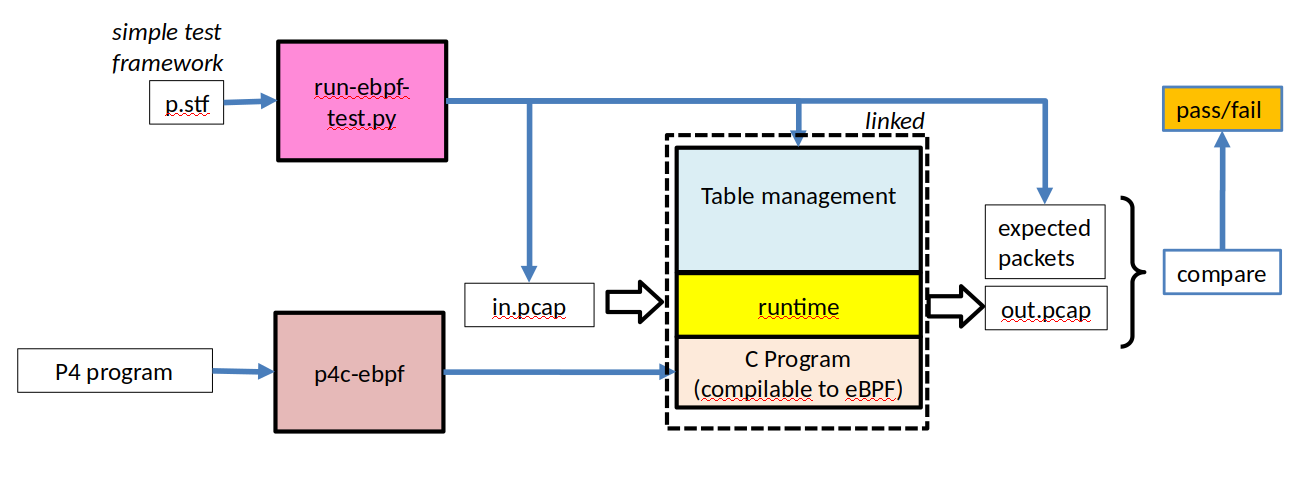
\includegraphics[width=\linewidth]{user_test}
	\caption{User-level testing of the C programs generated by the P4 compilers.}
	\label{fig:user_test}
\end{figure}

\begin{figure}
	\centering
	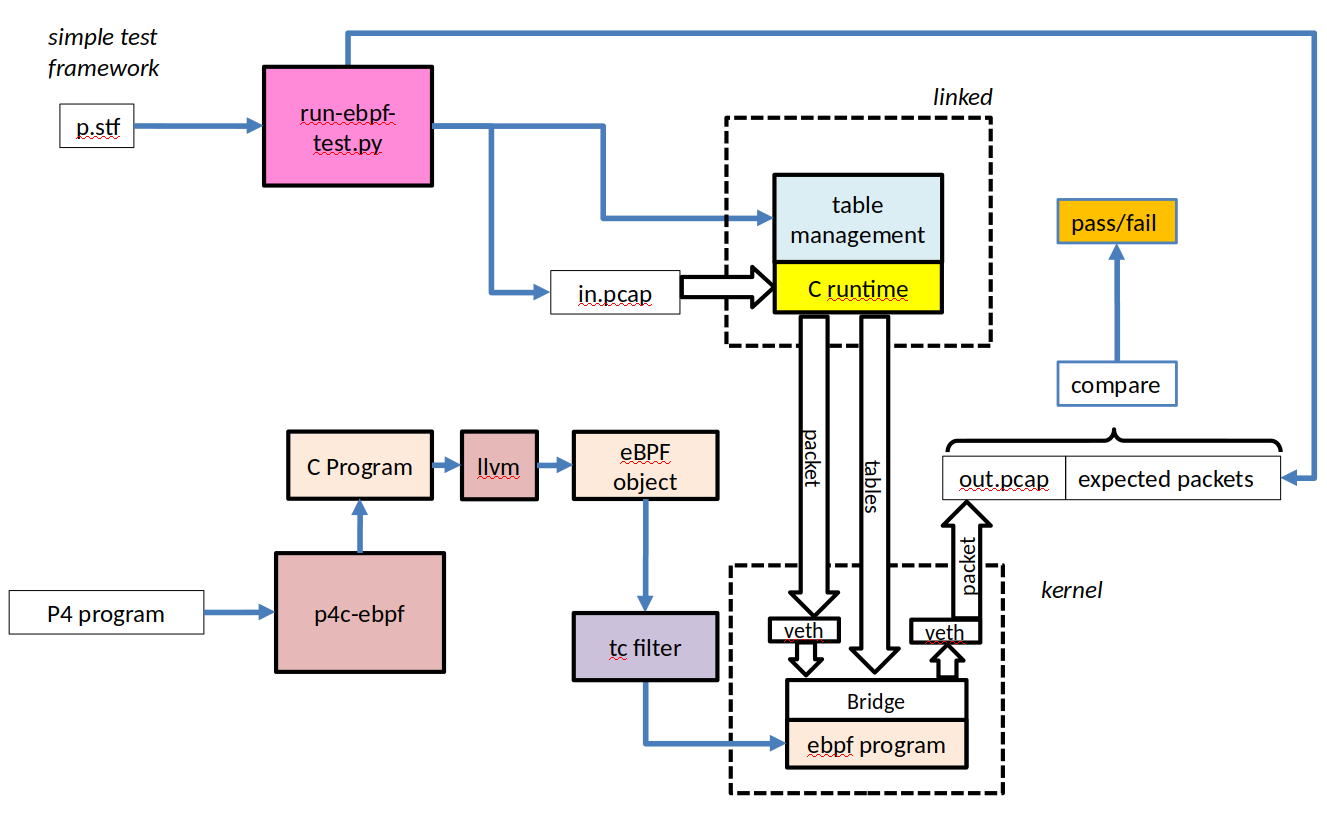
\includegraphics[width=\linewidth]{kernel_test}
	\caption{Kernel-level testing of the C programs generated by the P4 
	compilers.}
	\label{fig:kernel_test}
\end{figure}

\subsection{Using the test framework to compile eBPF/XDP programs}
The test framework can be used independently to verify eBPF and XDP programs. 


